\documentclass[11pt]{article}
\usepackage{scribe}
\usepackage{graphicx}

% Uncomment the appropriate line
%\Scribe{Your name}

\Scribes{Dino Mariano, Frendy Lio Can, Keenan Lee}
\LectureDate{December 2, 2020}
\LectureTitle{Final Report}

%\usepackage[mathcal]{euscript}

\addbibresource{references.bib}

\begin{document}

\MakeScribeTop

%\paragraph{This is a paragraph heading} Paragraph.

%%%%%%%%%%%%%%%%%%%%%%%%%%%%%%%%
% Introduction
%%%%%%%%%%%%%%%%%%%%%%%%%%%%%%%%
\paragraph{\noindent\textbf{\LARGE{Introduction}}}
\begin{flushleft}
    The goal of this project was to create and train a fully-connected network (FCN) 
    model (utilizing a pre-trained ResNet-50 base) to be able to classify CT-scans 
    of lungs into three categories, ``Healthy``, ``Other``, and ``Covid``. 
    \newline
    \newline
    The initial dataset consisted of $4171$ images, containing an uneven distribution
    of $757$ ``Healthy`` images, $1247$ ``Other`` images, and $2167$ ``Covid``images. 
    Dimensions between images differed significantly from each other.
\end{flushleft} 

%%%%%%%%%%%%%%%%%%%%%%%%%%%%%%%%
% Question A
%%%%%%%%%%%%%%%%%%%%%%%%%%%%%%%%
\paragraph{\noindent\textbf{\LARGE{Question a)}}}
\begin{flushleft}
    The question-box is filled by:
\end{flushleft} 
\begin{equation*}
\begin{split}
    x_i^{[2]} = & \sum_{j=1}^3 z_j^{[1]} * c_i^{[2]} \quad , x_i : i = 1, \cdots, 5
\end{split}
\end{equation*}
\begin{flushleft}
    The number of parameters is: $3*5*5$ (First Layer) + $5*5*5$ (Second Layer) $=200$.
\end{flushleft} 


%%%%%%%%%%%%%%%%%%%%%%%%%%%%%%%%
% Question C
%%%%%%%%%%%%%%%%%%%%%%%%%%%%%%%%
\paragraph{\noindent\textbf{\LARGE{Question c )}}}
\paragraph{\noindent\textbf{\LARGE{Pre-processing}}}
\begin{flushleft}
    Before training, several operations were performed on the images. 
    All images were resized to $224$x$224$ and converted to grayscale. 
    The reason for this resizing was to meet ResNet-50 requirements of a $3$x$224$x$224$
    image and was performed via scaling using the resize function of the OpenCV 
    library. 
    \newline
    \newline
    We chose to scale the images, as we found that cropping would result
    in the loss of too much information. The grayscale transformation was for 
    transportability. The training was done on the Google Colab platform and 
    new sessions required a re-import and processing of data, so saving images as 
    grayscale made everything quicker. 
    \newline
    \newline
    Input images were also augmented, with all images being rotated three times 
    $(90, 180, $ and $270)$ as well as being flipped horizontally to increase 
    the size of the dataset. 
    \newline
    \newline
    To improve our data, we could have performed additional augmentation to the 
    ``Healthy`` and  ``Other`` images, which would have evened out the distribution 
    of data; however, we were not able to do so due to time constraints.
    \newline
    \newline
    When training the model, we needed to include five-fold cross-validation. 
    To load the data into our model, we first split the images into $5$ different 
    folders. The split was done randomly, and each class of image was split separately 
    to ensure a uniform distribution of classes across splits. Labels were stored 
    in a CSV, and each folder was loaded as a separate dataset. 
    \newline
    \newline
    To implement our five-fold cross-validation, we created five separate train/test 
    sets, concatenating four of the datasets for training and using the last dataset
    as the testing split.  
    \newline
    \newline    
    When images were loaded into our dataset class, two duplicate channels were 
    added to each image, bringing the image to the required $3$x$224$x$224$ from the 
    original $1$x$224$x$224$. 
    \newline
    \newline
    Additionally, images were normalized and standardized. 
    Mean and the standard deviation were calculated individually for each of 
    the 5 datasets. This was done for convenience, as we found that the 
    recommended way, standardizing both training and testing data on 
    values of mean and standard deviation calculated from the training set \cite{Medium},
    was difficult with our implementation of five-fold cross-validation. 
    \newline
    \newline
    We found this method acceptable because it did not result in data leakage 
    and we found that the mean and standard deviation across different datasets 
    varied by only around $\pm 0.003$.
\end{flushleft} 

%%%%%%%%%%%%%%%%%%%%%%%%%%%%%%%%
% PROBLEM 1 C
%%%%%%%%%%%%%%%%%%%%%%%%%%%%%%%%
\paragraph{\noindent\textbf{\LARGE{ResNet-50}}}
\begin{flushleft}
    We found that the best results where by freezing the first 7 children 
    of the pre-trained ResNet-50 model. Increasing the number of frozen children 
    led to a lower accuracy while freezing less led to the model overfitting 
    much quicker with lower testing accuracy.
\end{flushleft} 
    

%%%%%%%%%%%%%%%%%%%%%%%%%%%%%%%%
% PROBLEM 2 A
%%%%%%%%%%%%%%%%%%%%%%%%%%%%%%%%
\paragraph{\noindent\textbf{\LARGE{Forward Network}}}
\begin{flushleft}
    Our final Feed Forward Network consisted of three linear layers, 
    separated by batch normalization and ReLU layers. 
    We learnt that applying batch normalization after the activation function is a 
    general rule \cite{Normalization}. 
    \newline
    \newline
    In our case, we found no significant difference between placing 
    batch normalization layers before or after ReLU. We did, however, 
    achieve slightly better accuracy placing batch normalization before the ReLU 
    function; thus, our final model consisted of the following: 
    \begin{enumerate}
        \item Linear layer
        \item Batch normalization
        \item ReLU
        \item Linear layer
        \item Batch normalization
        \item ReLU
        \item Linear layer
    \end{enumerate}
    We decided on a model with three linear layers as we found that (without tuning) 
    only having two layers led to major underfitting, and having four linear layers 
    led to quick overfitting and low overall accuracy.
\end{flushleft} 

%%%%%%%%%%%%%%%%%%%%%%%%%%%%%%%%
% PROBLEM 2 B
%%%%%%%%%%%%%%%%%%%%%%%%%%%%%%%%
\paragraph{\noindent\textbf{\LARGE{Optimizer}}}
\begin{flushleft}
    In our final model, we decided to use Stochastic Gradient Descent (SDG) as 
    our optimizer (with momentum $=0.2$). However, we were able to achieve more than $85\%$ 
    accuracy with both ADAM and SDG, so our reason for choosing SDG was not 
    based on anything significant.
\end{flushleft} 
%%%%%%%%%%%%%%%%%%%%%%%%%%%%%%%%
% PROBLEM 2 C
%%%%%%%%%%%%%%%%%%%%%%%%%%%%%%%%
\paragraph{\noindent\textbf{\LARGE{Loss Function}}}
\begin{flushleft}
    We kept the default Cross-Entropy Loss function. 
\end{flushleft} 

%%%%%%%%%%%%%%%%%%%%%%%%%%%%%%%%
% PROBLEM 2 D
%%%%%%%%%%%%%%%%%%%%%%%%%%%%%%%%
\paragraph{\noindent\textbf{\LARGE{Hyperparameters}}}
\begin{flushleft}
    After trial and error, we concluded the following:
\begin{itemize}
    \item Batch Size: 32
    \item Number of neurons in layer 1 (l1Tol2Features): 96
    \item Number of neurons in layer 2 (l2tol3Features): 64
    \item Epochs: 10
    \item Learning rate: 0.08
    \item The number of children frozen in ResNet-50: 7
    \item Momentum: 0.2
\end{itemize}    
\end{flushleft} 

%%%%%%%%%%%%%%%%%%%%%%%%%%%%%%%%
% PROBLEM 2 E
%%%%%%%%%%%%%%%%%%%%%%%%%%%%%%%%
\paragraph{\noindent\textbf{\LARGE{Data}}}
\begin{flushleft}
    Our best model had an average accuracy of $ 90.6 \% $.
\end{flushleft} 

\begin{figure}[H]
    \centerline{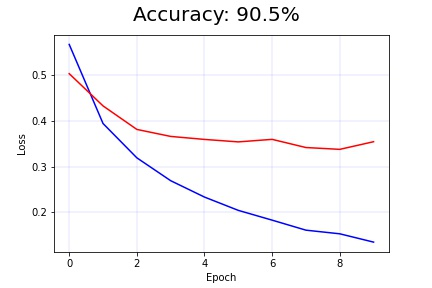
\includegraphics[scale=.5]{image1.jpg}}
    \caption{First fold}
    \label{fig}
\end{figure}

\begin{figure}[H]
    \centerline{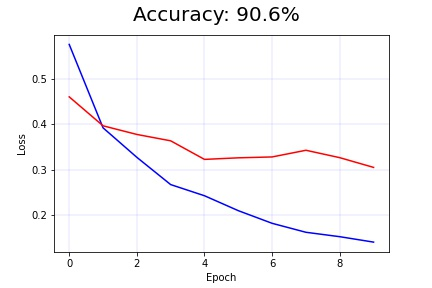
\includegraphics[scale=.5]{image2.jpg}}
    \caption{Second fold}
    \label{fig}
\end{figure}

\begin{figure}[H]
    \centerline{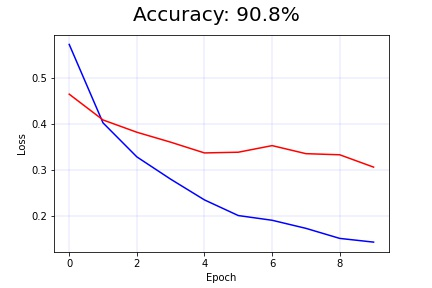
\includegraphics[scale=.5]{image3.jpg}}
    \caption{Third fold}
    \label{fig}
\end{figure}

\begin{figure}[H]
    \centerline{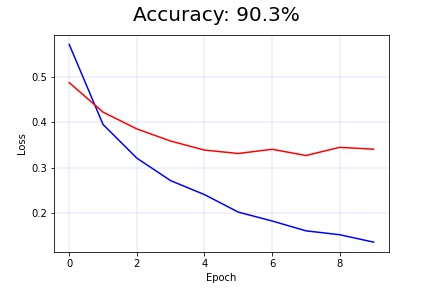
\includegraphics[scale=.5]{image4.jpg}}
    \caption{Fourth fold}
    \label{fig}
\end{figure}

\begin{figure}[H]
    \centerline{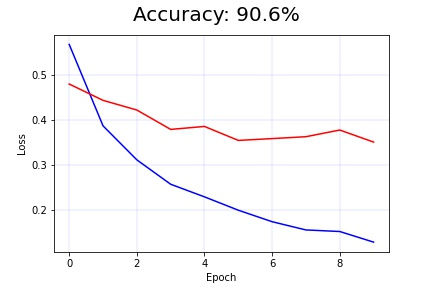
\includegraphics[scale=.5]{image5.jpg}}
    \caption{Fifth fold}
    \label{fig}
\end{figure}

%%%%%%%%%%%%%%%%%%%%%%%%%%%%%%%%
% PROBLEM 2 F
%%%%%%%%%%%%%%%%%%%%%%%%%%%%%%%%
\pagebreak
\printbibliography
\end{document}
